% fancytikzposter.tex, version 2.1
% Original template created by Elena Botoeva [botoeva@inf.unibz.it], June 2012
% 
% This file is distributed under the Creative Commons Attribution-NonCommercial 2.0
% Generic (CC BY-NC 2.0) license
% http://creativecommons.org/licenses/by-nc/2.0/ 


\documentclass{a0poster}

\usepackage{fancytikzposter_sources/fancytikzposter} 


%%%%% --------- Change here if you want ---------- %%%%%
%% margin for the geometry package, must be changed before using the geometry package
%% default value is 4cm
\setmargin{2}

%% the space between the blocks
%% default value is 2cm
% \setblockspacing{2}

%% the height of the title stripe in block nodes, decrease it to save space
%% default value is 3cm
% \setblocktitleheight{3}

%% the number of columns in the poster, possible values 2,3
%% default value is 2
\setcolumnnumber{3}

%% the space between two or more groups of authors from different institutions
%% used in \maketitle
% \setinstituteshift{10}

%% which template to use
%% N1 simple, standard look, with a colored background and gray boxes
%% N2 board with nodes
%% N3 another standard look
%% N4 envelope-like look
%% N5 with a wave-like head, original idea taken from
%%%% http://fc09.deviantart.net/fs71/f/2010/322/1/1/scientific_poster_by_nabuy-d333ria.jpg
%\usetemplate{3}

%% components of the templates
%% (the maximal possible numbers are mentioned as the parameters)
% \usecolortemplate{4}
% \usebackgroundtemplate{5}
% \usetitletemplate{2}
% \useblocknodetemplate{5}
% \useplainblocktemplate{4}
% \useinnerblocktemplate{2}


%% the height of the head drawing on top 
%% applicable to templates N3, 4 and 5
% \setheaddrawingheight{14}


%% change the basic colors
%\definecolor{myblue}{HTML}{008888} 
%\setfirstcolor{myblue}% default 116699
%\setsecondcolor{gray!80!}% default CCCCCC
%\setthirdcolor{red!80!black}% default 991111

%% change the more specific colors
% \setbackgrounddarkcolor{colorone!70!black}
% \setbackgroundlightcolor{colorone!70!}
\setbackgrounddarkcolor{colorone!70!}
\setbackgroundlightcolor{colorone!70!black}
% \settitletextcolor{textcolor}
% \settitlefillcolor{white}
% \settitledrawcolor{colortwo}
% \setblocktextcolor{textcolor}
% \setblockfillcolor{white}
% \setblocktitletextcolor{colorone}
% \setblocktitlefillcolor{colortwo} %the color of the border
% \setplainblocktextcolor{textcolor}
% \setplainblockfillcolor{colorthree!40!}
% \setplainblocktitletextcolor{textcolor}
% \setplainblocktitlefillcolor{colorthree!60!}
% \setinnerblocktextcolor{textcolor}
% \setinnerblockfillcolor{white}
% \setinnerblocktitletextcolor{white}
% \setinnerblocktitlefillcolor{colorthree}




%%% size of the document and the margins
%% A0
\usepackage[margin=\margin cm, paperwidth=118.9cm, paperheight=84.1cm]{geometry} 
% \usepackage[margin=\margin cm, paperwidth=84.1cm, paperheight=118.9cm]{geometry}
%% B1
% \usepackage[margin=\margin cm, paperwidth=70cm, paperheight=100cm]{geometry}



%% changing the fonts
\usepackage{cmbright}
%\usepackage[default]{cantarell}
%\usepackage{avant}
%\usepackage[math]{iwona}
\usepackage[math]{kurier}
\usepackage[T1]{fontenc}


%% add your packages here
\usepackage{hyperref}
\usepackage{tipa}


\title{Evaluation of Speech Enhancement and Practical Speech Enhancement in Babble Using Phoneme-Dependent Non-negative Matrix Factorisation}
\author{Ashley Gillman\\
  \texttt{ashley.gillman@my.jcu.edu.au}\\
  James Cook University, Townsville
  \And
  Dr. Owen Kenny\\
  \texttt{owen.kenny@jcu.edu.au}\\
  James Cook University, Townsville
}


\begin{document}

%%%%% ---------- the background picture ---------- %%%%%
%% to change it modify the macro \BackgroundPicture
\ClearShipoutPicture
\AddToShipoutPicture{\BackgroundPicture}

\noindent % to have the picture right in the center
\begin{tikzpicture}
  \initializesizeandshifts
  % \setxshift{15}
  % \setyshift{2}


  %% the title block, #1 - shift, the default value is (0,0), #2 - width, #3 - scale
  %% the alias of the title block is `title', so we can refer to its boundaries later
  \ifthenelse{\equal{\template}{1}}{ 
    \titleblock{80}{1}
  }{
    \titleblock{47}{1.5}
  }

  %% a logo can be added to the title block
  %% #1 - anchor relative to the title block, #2 - shift, #3 - width, #3 - file name
  % \ifthenelse{\equal{\template}{2}}{ 
     \addlogo[south west]{(-15,-65)}{15cm}{fig/JCU_Logo_MONO_REV.eps}
  % }{
  %   \addlogo[south west]{(2,0)}{6cm}{unibz_w.png}
  % }

  \blocknode%
  {Speech Enhancement}%
  {
  There are many reasons to enhance speech, including applications for the hearing impaired, telecommunications, and improving automated speech recognition (ASR) systems.

  \begin{center}\begin{minipage}{0.9\linewidth}
    \vspace{1cm}\innerblockplain[colorone!80!]{
    Imagine a hearing system that could recognise and extract specific voices. A child could train their cochlear implant to recognise their Mother's voice to hear her easily even in a busy shopping center. An elderly woman could `tune' her hearing aid into her husband's voice to hear him at a cafe.

    Or imagine a mobile phone that could filter out your voice so you can use it in a crowded place and still be heard. Or a speech recognising phone that worked regardless of where you are.
    }
  \end{minipage}\end{center}
%  }

%  \blocknode%
%  {Evaluation of Speech Enhancement}%
%  {
  
  In general, there are two types of applications for speech enhancement, those for humans (hearing devices, recordings, etc.) and those for machines (improving ASR quality). But these two types of listeners `hear' is very different ways.

  However, usually when a new enhancement algorithm is proposed, this fact is ignored. Shown below in Figure \ref{fig:assessmentMethods} are some of the methods used to measure speech enhancement.

  \begin{tikzfigure}[How speech enhancement is measured\label{fig:assessmentMethods}]
    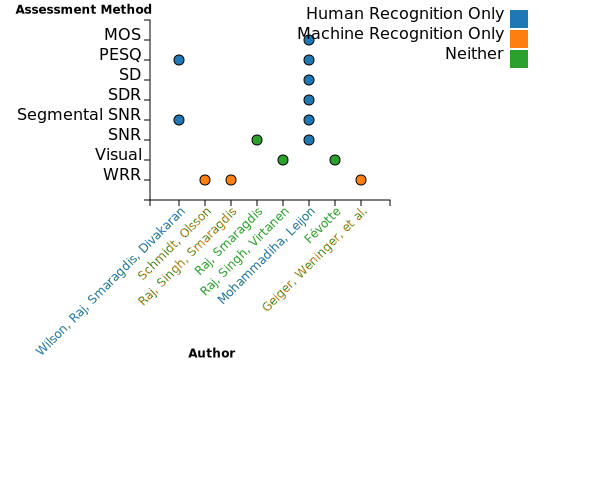
\includegraphics[width=0.8\textwidth]{fig/assessmentMethods.pdf}
  \end{tikzfigure}

  It can be seen that only one of the above papers considered both human and machine measures. This highlights the need to investigate the differences between when enhancement is measured for humans and machines.
  }

%  \blocknode%
%  {Contact}%
%  {\coloredbox{colorthree!50!}{
%    \begin{minipage}{0.5\linewidth}
%      Ashley Gillman\\
%      James Cook University, Townsville\\
%      \texttt{ashley.gillman@my.jcu.edu.au}
%    \end{minipage}
%    \begin{minipage}{0.5\linewidth}
%      Dr. Owen Kenny\\
%      James Cook University, Townsville\\
%      \texttt{owen.kenny@jcu.edu.au}
%    \end{minipage}
%    }
%  }
  
  \startsecondcolumn

  \blocknode%
  {Evaluation of Speech Enhancement}%
  {An investigation was conducted in which a number of enhancement algorithms were measured using a number of enhancement measurement techniques. These techniques included the correctness and accuracy of an ASR system, where an ASR system was implemented and the correctness (percentage phonemes recognised) and accuracy (percentage phonemes recognised, minus any false insertions).
  Also included was the comparative mean opinion score (MOS) test, where human listeners are asked to rate the level of enhancement.

  Figure \ref{fig:Hum-Mac-Res} below shows the enhancement for machines on the x-axis (correctness and accuracy improvement) and enhancement for humans on the y-axis.

  \begin{tikzfigure}[Human vs. machine enhancement\label{fig:Hum-Mac-Res}]
    \includegraphics[width=0.5\textwidth]{fig/cmos-prrcorrimp.pdf}\includegraphics[width=0.5\textwidth]{fig/cmos-prraccimp.pdf}
  \end{tikzfigure}

  Results indicated that there was some correlation between human and machine recognition measured as correctness, but not when measured as accuracy.
  Furthermore, multiple occurrences were noted where enhancement algorithms were found to be much more suited to either human or machine hearing.

  It was concluded that both human and machine measures are required to classify the performance of an enhancement algorithm. Specific measures recommended are the perceptual evaluation of speech quality measure (PESQ) as a human measure, for its ease of implementation; a MOS test where possible, subject to available funding; and the word recognition rate of an ASR system, or if possible multiple ASR systems.
  }

  \blocknode%
  {Phonemic Modifications to NMF Algorithms}%
  {Non-negative matrix factorisation is a form of matrix decomposition, that decomposes a non-negative matrix (i.e. all values are 0 or greater) into two separate matrices, as illustrated in Figure \ref{fig:nmf}. NMF is notable for its ability to draw out the `parts' of a system, and can factorise a matrix into $V$, the parts or bases, and $W$, their occurrences or activations.

  \begin{tikzfigure}[Non-negative matrix factorisation\label{fig:nmf}]
    \includegraphics[width=0.7\textwidth]{fig/nmf.eps}
  \end{tikzfigure}
  }
  
  \startthirdcolumn

  \blocknode%
  {Phonemic Modifications to NMF Algorithms Cont.}%
  {
  Phonemes are the building blocks of speech. Figure \ref{fig:phoneme} visualises speech being broken down into the individual components, the phonemes.

  \begin{tikzfigure}[Breaking speech down into phonemes\label{fig:phoneme}]
  \begin{center}\begin{tabular}{r | l}
    Phrase & ``Examine a sentence.'' \\
    Words & ``Examine'' + ``a'' + ``sentence'' \\
    Syllables & /Ex.am.ine/ + /a/ + /sen.tence/ \\
    %Phonemes & (IH G Z AE M IH N) + (AH) + (S EH N T EH N S) \\
    Phonemes & \textipa{/I g z \ae{} m I n/ + /9/ + /s E n t E n s/} \\
  \end{tabular}\end{center}
  \end{tikzfigure}

  The motivation for forming phoneme-dependent NMF is drawn from the fact that NMF algorithms attempt to pull out the `parts' of speech, and our most atomic `parts' of speech are the phonemes.

  The proposed modification was to replace the training data used to train the algorithm to a specific voice. This is typically sentences read by the speaker, but in this proposed phonemic training method is a specified number of samples of each phoneme concatenated together. This forms high density training data, eliminating the transient silences in the speech.
  }

  \blocknode%
  {Performance of Phoneme-Dependent NMF}%
  {Figure \ref{fig:Hum-Mac-Res} below shows the enhancement for machines on the x-axis (correctness and accuracy improvement) and enhancement for humans on the y-axis. So points above the diagonal line indicate improvement by using phoneme-dependent training.

  \begin{tikzfigure}[Human vs. machine enhancement\label{fig:Hum-Mac-Res}]
    \includegraphics[width=0.4\textwidth]{fig/CMOS.pdf} \includegraphics[width=0.4\textwidth]{fig/PRRaccImp.pdf}
    \includegraphics[width=0.9\textwidth]{fig/leg.pdf}
  \end{tikzfigure}

  On the left are shown the results for humans and on the right results for machines. It was noted that there were no significant differences for these algorithms for humans, however there was, in general, a slight increase for machines. There were some algorithms that performed much better for machines, in particular those corresponding to car noise. However those corresponding to a same-sex competing speaker noise performed poorer.

  It was concluded that phoneme-dependent training methods are a viable option for enhancement for ASR systems. Since the modifications are easily to implement, they could be investigated on a case-by-case basis for possible integration.

  Additionally, these tests highlighted the importance of the previous investigation into human vs. machine enhancement performance. It was seen in these tests that performance varied significantly depending on test measures utilised.
  }


\end{tikzpicture}
\end{document}




